%\chapter{Spatial Capture-Recapture for Unmarked Populations}
\chapter{Unmarked Populations}
\markboth{Chapter 14 }{}
\label{chapt.scr-unmarked}

\vspace{0.3cm}

%\hl{todo: Royle-Nichols observaiton model}

Traditional capture-recapture models share the fundamental
assumption that each individual in a population can be uniquely
identified when captured. Oftentimes this can be accomplished
by marking individuals with color bands, ear tags, or some other
artifical mark that can be subsequenly read in the field. For other
species, such as tigers (\textit{Panthera tigris}) or
marbled salamanders (\textit{Ambystoma opacum}),
individuals can be easily identified
using only their natural markings. However, many species
do not possess adequate natural markings and are
difficult to capture, making it impractical to use standard
capture-recapture techniques.

Estimating density when individuals are unmarked can be accomplished
using a variety of alternatives to capture-recapture, such as distance
sampling \citep{buckland_etal:2001} and $N$-mixture models
\citep{royle:2004biom}. These methods, and others, can be
very effective when their assumptions are met, but in cases such as
when it is not possible to obtain accurate distance data, or when
movement complicates the use of fixed-area plots,
these methods may not yield unbiased estimates of density
\citep{chandler_etal:2011}. In this chapter we highlight the work of
\citet{chandler_royle:2012} who demonstrated that the ``individual
recognition'' assumption of traditional capture-recapture models is not a
requirement of spatial capture-recapture models. They showed that,
under certain conditions described below, spatially-correlated count
data are sufficient for making inference about animal distribution and
density even when no individuals are marked.
The \citet{chandler_royle:2012} ``spatial count model'' (hereafter the SC
model) require neither distance data nor fixed area plots. Instead,
the observed data are trap- and occasion-specific counts, which
are modeled as a reduced-information summary of the \textit{latent}
encounter histories. Because the model is formulated in terms of the
data we wish we had, i.e. the typical encounter history data observed
in standard capture-recapture studies of marked animals, the SC model
is just a SCR model with a single extension to account for the fact
that the encounter history data are unobserved.
%To be more precise, we model the counts as:
%$n_{jk} = \sum_i y_{ijk}$ where $n_{jk}$ is the count data and
%$y_{ijk}$ is the encounter history data. Thus, the model
%is virtually identical to standard SCR models except that the
%encounter histories $\{y_{ijk}\}$ are not directly observed.

The ability to fit SCR models to data from unmarked populations has
important implications. For one, it means that SCR models can
be applied to data collected using methods like points counts in which
observers record simple counts of animals at an array of survey
points. The model can also be fit to camera trapping data collected on
unmarked animals, and prior to the SC models
there were few, if any, options for modeling density from such data.
So, is this model a free lunch? At face value, it sounds as though we
can estimate all the quantities of interest in standard
capture-repature studies, but with very little
data. The answer is of course not---lunch is still not free because
with this model come new assumptions,
which we will describe in this chapter,
and as was demonstrated by
\citet{chandler_royle:2012}, even with ``perfect'' data, the estimates
will typically not be as precise as might be hoped for. This should
not be surprising given that we are asking so much from simple count
data.

The real value of the SC model is two-fold. First, it demonstrates
an important theoretical result %, namely,
that spatial correlation in
count data carries information about the distribution of
individuals. This stands in stark contrast to a prevailing view of
spatial correlation as a nuisance to be avoided or modeled out of unsightly
residual plots. The second reason why this model is important is that
it provides the basis for handling the extremely common phenomenon in
which not all individuals in a population can be marked or otherwise
distinguishable. Thus, while we do not recommend foregoing the work
required to mark animals, this model does provide a method for
studying unmarked populations, which \textit{can} yield precise
density estimates if some of the individuals are marked, or if prior
information about some of the parameters is available.
The extension of this model to handle data from marked and unmarked
individuals is thoroughly treated in the next chapter. Here, we focus
on the case in which all individuals are unmarked.

\section{Existing Models for Inference About Density in Unmarked Populations}
\label{Sect.existing-unmarked}

When capture-recapture methods are not a viable option, ecologists
often collect simple count data or even binary detection/non-detection data
to estimate parameters such abundance or occupancy.
%\citep{royle:2004biom, mackenzie_etal:2002}.
These
data may be analyzed using generalized linear models such as
Poisson regression or logistic regression, perhaps with random
effects. %When detection is imperfect, as it almost always is,
However, these methods will be biased when detection is imperfect, as
it usually is. Even when count data or detection/non-detection data are
used as an index of abundance or occurrence, standard models may yield
unreliable results when covariates affect both the ecological process
and the observation process. A classic example is given by
\citet{bibby_buckland:1987} who found that songbird detection
probability was negatively related to vegetation height, whereas
density was positively associated with vegetation height in restocked
confier plantations. This intuitive phenomenon has been
found demonstrated repeatedly \citep[e.g.][]{kery:2008,sillett_etal:2012} and has led to the
development of a vast number of models to estimate population size and
detection probability when individuals are unmarked. A review of these
models is beyond the scope of this
chapter, but we mention a few deficiencies of existing methods
that warrant the exploration of alternatives for robust inference when
standard capture-recapture methods do not apply.

Distance sampling \citep{buckland_etal:2001}, which we briefly
introduced in Chapter~\ref{chapt.intro},
is perhaps the most widely used method for
estimating population density when individuals are unmarked and
detection probability is less than one. This class of methods is known
to work impecibly when estimating the number of stakes in a field or
the number of duck nests in a wetland. Distance sampling can also work very well in
more interesting situations, and it is an extremely powerful method when
the assumptions can be met. However, the assumptions that distance
data can be recorded without error and that animals are distributed
randomly with respect to the transect can be easily violated by
common processes such as animal movement and measurement
error. Although numerous methods have been proposed to
relax some of these assumptions
\citet{royle_etal:2004, borchers_etal:1998, johnson_etal:2010,
  chandler_etal:2011},
another issue is that distance
sampling is simply not practical in many settings. For example, many
species are so rare and elusive that they can only be reliably
surveyed using methods such as camera traps.

Other common sampling methods used to estimate density when individuals are
unmarked include double-observer sampling, removal sampling, and
repeated counts, for which custom models have been developed
\citep{nichols_etal:2000, farnsworth_etal:2002, royle:2004biom,
  royle:2004abc, nichols_etal:2009,fiske_chandler:2011}. To
obtain reliable density estimates using these
methods, the area surveyed must be well defined and closed with
respect to movement and demographic processes. Given a sufficiently short
sampling interval, such as a 5-min point-count, the closure
assumption may be reasonable. However, short sampling intervals limit
the number of detections, so observers generally visit each survey
location multiple times during a season. But then, animal
movement may invalidate the closure assumption, and a model of
temporary emigration is required
\citep{kendall_etal:1997,chandler_etal:2011}. Furthermore,
distance-related heterogenity in detection probability can introduce
bias in these models, although this bias is negligible when the
ratio of plot size to the scale parameter of the detection function is low
\citep{efford_dawson:2009}.

We mention these issues not to suggest that existing models do not
have value---indeed we believe that they can be used to obtain
reliable density estimates in many situations---rather, our aim is to
highlight the need for alternative methods when the assumptions of
existing methods cannot be met and when spatially-explicit inference
is the objective. %Additionally, the spatial count model
%we discuss in this chapter serves as the foundation for a broad class
%of SCR models in which all or some of the individuals cannot be
%uniquely identified, which is the focus of the next chapter.


\section{Spatial Correlation as Information}
\label{sect.corr-info}

All of the previous methods require some sort of auxiliary information
to model both abundance and detection. For instance, we might
need multiple observers or distance data or repeated visits to ensure
that model parameters are identifiable (but see
  \citep{lele_etal:2012, solymos_etal:2012}). The same is true for
the SC model, but the auxiliary information comes in the form of spatial
correlation, which requires no extra effort to collect
\citep{chandler_royle:2012}. %In fact, it's probably safe to say that
%it is harder to avoid spatial correlation that it is to

It is natural to be suspicious of the claim that spatial correlation
is a good thing. Indeed, elaborate methods have been devised to deal
with spatial correlation as a nuisance parameter
\citep{lichstein_etal:2002,dormann_etal:2007}, and ecologists have been admonisted for
failing to obtain ``real'' replicates uncontaminated by spatial
correlation \citep{hurlbert:1984}. The following heuristic may be
helpful for seeing the value of spatial correlation.

Imagine a 10$\times$10 grid of camera traps and a single unmarked
individual exposed to ``capture'' whose home range center lies in the center of the
trapping grid. If the individual has a small home range size relative
to the extent of the trapping grid, we can imagine what the
spatial correlation structure of the encounters might look
like. If the animal's home range is symmetric around the activity center
then the number of times the individual is detected at each
trap (the trap count) is a function of the distance between the home
range center and the trap; i.e., traps with the same distance
from the activity center will yield counts that are more highly
correlated with one another than traps located at different distances
from the activity center. Thus, the correlation in counts tells us
something about the location of the activity center. It is relatively
intuitive that spatial correlation carries information about
distribution, but what about density?


Imagine now that there are two activity centers located in the traping
grid. Using trap counts alone, %which allow for imperfect detection,
is it possible to determine the number and location of these activity
centers? The answer is yes, at least under certain circumstances.
Figure~\ref{chapt-unmarked.fig.heur} illustrates the process. The
figure shows the locations of the two activity centers, and the total
counts made at each trap after 10 survey occasions.
%distance between the sampling location and the individual.
Assuming that animals have bivariate normal home
ranges, the fact that there are two areas in the map with high counts
that dissipate in both dimensions suggests that the most likely number of
individuals given these data is 2. Furthermore, the degree to which
the counts dissipate from the two areas of highest intensity is
information about the home range size parameter $\sigma$. These two
piecies of information are enough to estimate the number of
individuals exposed to sampling---again, given
that a bivariate normal home range is a valid assumption. Of course,
the data could just as well have been generated by a single individual
whose home range is distinctly biomodal, and thus \textit{as always}
the assumptions of our model need to be carefully examined using our
biological knowledge of the system.

\begin{figure}%[ht!]
\centering
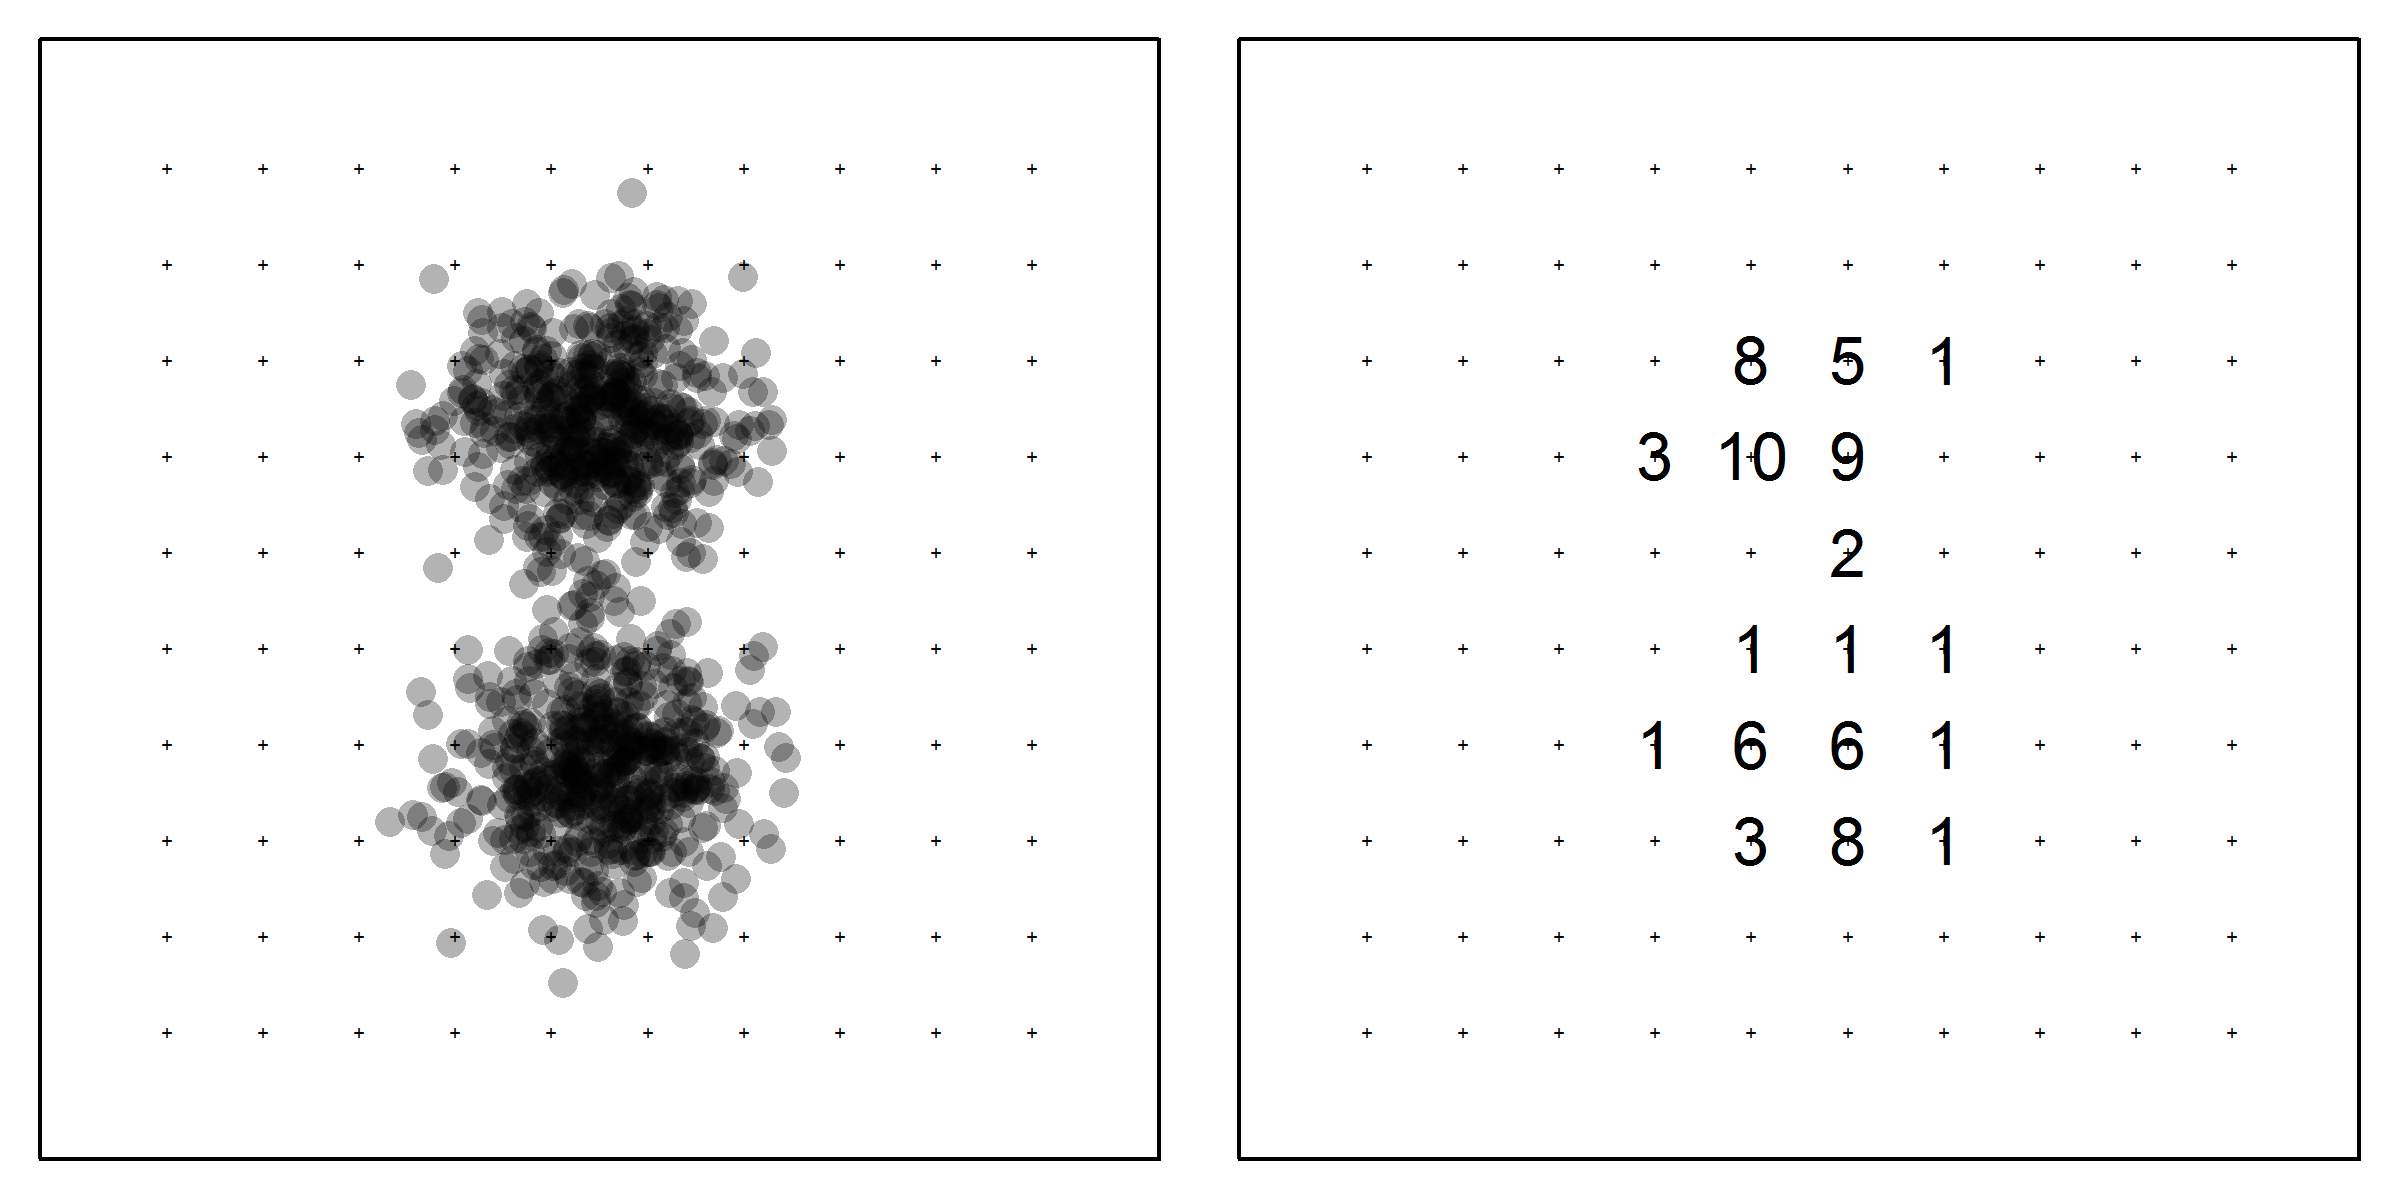
\includegraphics[width=0.5\textwidth]{Ch18-Unmarked/figs/heuristic}
\caption{Simulated count data at each of 100 camera traps
  (crosses) after $K=10$ sampling occasions. The circles are the
  locations of two animal activity centers. The
  \citet{chandler_royle:2012} model attempts to
  estimate both the location and number of activity centers exposed to
  sampling using only the spatially-referenced count data.}
\label{chapt-unmarked.fig.heur}
\end{figure}





\section{Data}

Whereas traditional SCR models require spatially-referenced
encounter histories, this model requires simple count data.
Let $n_{jk}$ be the count data at sampling locations $j$ %;
%j=1,\ldots J$
on occasion $k$. %; k=1,\ldots,K$.
The $J \times K$ matrix of
counts will be denoted $\bf{n}$. A sampling location in this context
could be any device capable of recording count data, such as a
human observer or a camera trap, and
one of the benefits of the SC model is that it
can be applied to data collected using many different survey
methods. For ease of presentation, we will refer to sampling devices
as traps, but remember that a trap is just something capable of
recording count data. As in all SCR models, we also require the
coordinates of the $J$ traps, and we denote the location of trap $j$
by ${\bf x}_j$. In some instances, additional data might be avialable such as
trap-specific covariates, state-space covariates,
information on the identities of a subset of individuals, or perhaps
even distance data, but in this chapter we ignore these %extraneous
possibilities so that we can focus on the basic model.

%The duration of sampling
%is assumed to be short enough such that the number of individuals
%exposed to sampling does not change over time.

\section{Model}

The state model is exactly the same as the one we have dealt with
throughout
this book. It is a point process describing the number and distribution of
activity centers in the state-space $\mathcal{S}$. Although it might
be possible to fit inhomogeneous point process models using the
methods described in Chapt.~\ref{chapt.state-space},
%we suspect thatpower to detect effects
given the simplicity of the data, we concentrate on a homogeneous point process
$\{{\bf s}_i, \ldots, {\bf s}_N\} \sim \text{Uniform}(\mathcal{S})$
where ${\bf s}_i$ is the activity center of individual $i$ in the
population of size $N$. For the moment, we will assume that $N$ is
known.

The observation model is the same as in other SCR models covered
in the sense that it describes the probability of encountering individual
$i$ at trap $j$, conditional on the location of the individual's
activity center. The specific encounter process will depend on the
sampling method, and here we consider the standard camera trapping
situation in which an individual can be encountered at multiple traps
during a single time period, say one night during a camera-trapping
study, and it can be detected multiple times at a single trap during
an occasion. This is the Poisson encounter model (a.k.a. the proximity
detector case) described in
Chapt.~\ref{chapt.poisson-mn}. As before, we define $y_{ijk}$ as the
encounter data for individual $i$ at trap $j$ on occasion $j$, which
we model as:
\begin{equation}
 y_{ijk} \sim \mbox{Poisson}(\lambda_{ij})
\label{eq.latentPoisson}
\end{equation}
where $\lambda_{ij}$ is the encounter rate. A common encounter rate model is the
Gaussian, or half-normal, model:
\[
\lambda_{ij} = \lambda_0 \exp(\| {\bf x_j - s_i} \| / 2\sigma^2)
\]
in which $\lambda_0$ is the baseline encounter rate, $\| {\bf x_j - s_i}
\|$ is the Euclidean distance between the trap and activity center, and $\sigma$ is the
scale parameter determining the degree to which encounter rate decreases with
distance.

When individuals cannot be uniquely identified, the encounter histories cannot
be directly observed, which seems like a massively insurmountable
problem. The solution of \citet{chandler_royal:2012} is the same one we routinely apply when we
cannot directly observe the process of interest---we regard the
encounter histories as latent variables. This leaves one remaining
task -- we need to specify the relationship between the count data and
the encounter histories, i.e we need a model of $[{\bf n}|{\bf y}]$
where $\bf y$ represents the entire collection of encounter
histories. In this case, there is only one possibility because, by
definition, the count data are simply a
reduced-information summary of the latent encounter histories. That
is, they are the sample- and trap-specific totals, aggregated over all
individuals:
\begin{equation}
n_{jk} = \sum_{i=1}^{N} y_{ijk}.
\label{chapt.unmarked.eq.ny}
\end{equation}
So, unlike most model-development problems faced in this book, we
don't have to consider competing probability models for
$[{\bf n}|{\bf y}]$, but instead, we honor the fact that the
relationship between the counts and the latent encounter histories is
deterministic. %You might think that extending the basic SCR model to
%include an additional deterministic component would not be too
%challenging...

%This data structure, a matrix of counts made at a collection of
%sampling locations on one or more occasions is extremely common in
%ecology. For example, think of avian point count data or camera
%trapping data from studies of unmarked animals.

Recall from Chapt.~\ref{chapt.modeling} that the sum of two or more
Poisson random variables is also a Poisson random variable.
Specifically,
if $x_1 \sim \text{Poisson}(\lambda_1)$ and
$x_2 \sim \text{Poisson}(\lambda_2)$, then $(x_1+x_2) \sim
\text{Poisson}(\lambda_1 + \lambda_2)$. Thus,
under this Poisson model for the latent encounter histories,
the count data can be modeled as Poisson:
\begin{equation}
n_{jk} \sim \mbox{Poisson}( \Lambda_{j} )
\label{eq:nagg}
\end{equation}
where
\[
 \Lambda_{j} = \lambda_0 \sum_{i} \exp(\| {\bf x_j - s_i} \| / 2\sigma^2),
\]
and because $\Lambda_j$ does not depend on $k$, we can
aggregate the replicated counts, defining
$n_{j.} = \sum_{k} n_{jk}$ and then
\[
 n_{j.} \sim \mbox{Poisson}( K \Lambda_{j} ).
\]
As such, $K$ and $\lambda_{0}$ serve equivalent roles as affecting
baseline encounter rate.

This formulation of the model in terms of the aggregate count
simplifies computations as the latent variables
$y_{ijk}$ do not need to be updated in the MCMC estimation
scheme; however, retaining $y_{ijk}$ in the formulation of the model
is important if some individuals are uniquely marked. %(Chapt.~\ref{chapt.partialID}).
This is because
uniquely identifiable individuals produce
observations of some of the $y_{ijk}$ variables, which we elaborate
on in the subsequent chapter.

Formulating the model in terms of the aggregated count data, $n_{j.}$,
demonstrates that the model can be
applied to data from a single sampling occassion $J \equiv 1$, as has
been noted elsewhere for standard SCR models
\citep{efford_etal:2009ecol}. In the context of studying marked
populations, the model parameters will only be identifiable in the
$J\equiv 1$ case if an animal can be captured at multiple traps during
a single occasion. The SC model essentially requires the same thing,
which is to say that it requires correlation in the count data
resulting from an individual being captured in multiple,
closely-spaced traps.


\subsection{On $N$ being unknown}
\label{chapt.unmarked.sec.N}

Population size, $N$, is never known in practice, and to estimate it,
we need a model for it. For homogeneous point process models,
$N$ is typically modeled as
$N \sim \text{Poisson}(\mu|\mathcal{S}|)$ or
$N \sim \text{Binomial}(M, \psi)$, the latter of which is equivalent
to a discrete uniform prior if $\psi \sim \text{Unif}(0,1)$. In
Chapt.~\ref{chapt.statespace} and elsewhere, we demonstrated that
the choice of prior has very little influence on parameter estimates,
and so we favor the binomial prior because of its convienence when
using MCMC -- it allows us to fix the
dimensions of the parameter space by setting $M$ to some arbitrarily
large integer.

A binomial model is
equivalent to a series of $M$ independent Bernoulli trials, and so
we can rewrite $N \sim \text{Binomial}(M, \psi)$ as $z_i \sim
\text{Bernoulli}(\psi)$ where $z_i$ is an auxilliary variable
indicicating if individual $i$ is a member of the population, i.e. $N =
\sum_{i=1}^M z_i$. Having expanded the model to include a prior on $N$, we
can summarize the SC model, with a Gaussian observation model, as follows:
\begin{align*}
  z_i &\sim \text{Bern}(\psi) \\
  y_{ijk} &\sim \text{Poisson}(\lambda_{ijk} z_i) \\
  \lambda_{ijk} &= \lambda_0\exp(-\|{\bf x}_j - {\bf s}_i\|^2)/(2\sigma^2) \\
  n_{jk} &= \sum_{i=1}^M y_{ijk} %\\
%  N &= \sum_{i=1}^M z_i
\end{align*}

%We note that there are actually two forms of data augmentation going
%on here: (1) we have our usual $M$ instead of $N$ model, and (2) from
%the perspective of modeling count data, we have augmented the model
%with


%\subsection{Inference}

Bayesian analysis can proceed once suitable priors have been put on
the hyperparamters $\psi$, $\sigma$, and
$\lambda_0$. \citet{chandler_royle:2012} provided \R~code for fitting
the model using MCMC, and they evaluated the model's performance with
uniform priors on the three hyperparameters. They also discussed the
possibilities and effects of including prior knowledge about $\sigma$
into the model. In the next section, we explain how the model can be
fit using \jags, but first we contemplate the viability of classical
analysis of this model.

The obvious challenge faced when conducting a classical analysis of
this model is that the number of latent variables in huge. In all SCR models, the activity centers are
latent, but now even the encounter histories are latent.
Maximizing likelihoods with latent variables (random effects) involves
integrating (or summing) over all possible values of the latent
variables. For the activity centers, this is typically accomplished by
integrating the conditional-on-$\bf s$ likelihood $[{\bf y}_i|{\bf s}_i]$ over the two-dimensional
state-space $\mathcal{S}$ (Chapt.~\ref{chapt.mle}). However, with
the SC model, we have to sum
over all possible encounter histories $\mathcal{H}$ meeting the
constraint of Eq.~\ref{chapt.unmarked.eq.ny}. The
number of possible encounter histories
%that could give rise to the count data
will, in general, be too high to make the likelihood tractible,
and thus we do not think that maximum likelihood is a viable option
for analyzing this model. However, one might be able to obtain maximum
likelihood estimates using simulation-based methods
%\citep{doucet_etal:2002,lele_etal:2010},
\citep{lele_etal:2010},
which will typically be more computationally
challenging than the MCMC-based Bayesian analysis.


\section{Simulation Example}

Simulating data under the SC model proceeds by first simulating
standard SCR encounter history data and then collapsing it into count
data. The following blocks of \R~code generate data from
the model shown in Sec.~\ref{chapt.unmarked.sec.N}, with parameters
$\sigma=0.04$, $\lambda_0=0.3$, and $N=50$. The state-space is the unit
square and a grid of 100 traps
is centered in the middle. These simulated data might resemble actual
data from a camera trap study in which an individual can be detected multiple
times at a trap during a single occasion, and at multiple traps during
an occasion. The first block of code generates the trap coordinates
$X$ and the $N=50$ activity centers:
\begin{verbatim}
> tr <- seq(0.3, 0.7, length=10)
> X <- cbind(rep(tr, each=length(tr)),
+            rep(tr, times=length(tr)))    # trap coords
> set.seed(10)
> xlim <- c(0, 1); ylim <- c(0, 1)         # S is the unit square
> A <- (xlim[2]-xlim[1])*(ylim[2]-ylim[1]) # area of S
> mu <- 50                                 # density (animals/unit area)
> (N <- rpois(1, mu*A))                    # Generate N=50 as Poisson deviate
[1] 50
> s <- cbind(runif(N, xlim[1], xlim[2]), runif(N, ylim[1], ylim[2]))
> plot(X, xlim=xlim, ylim=ylim, pch="+")
> points(s, col=gray(0.5), pch=16)
\end{verbatim}
We could have just set $N=50$ directly, but instead we treated density
as a fixed parameter ($\mu=50$) and generated $N$ as a random
variable -- it just so happens that with the specified random seed,
$N$ equals 50! % Once again, this highlights that fact that $N$ can be
% regarded as either a fixed or a random variable.

Now we can generate the encounter histories under the
Poisson observation model. Let's suppose that sampling is conducted
over $K=5$ nights.
\begin{verbatim}
> sigma <- 0.1
> lam0 <- 0.5
> J <- nrow(X)
> K <- 5
> y <- array(NA, c(N, J, K))
> for(j in 1:J) {
+     dist <- sqrt((X[j,1]-s[,1])^2 + (X[j,2] - s[,2])^2)
+     lambda <- lam0*exp(-dist^2/(2*sigma^2))
+     for(k in 1:K) {
+         y[,j,k] <- rpois(N, lambda)
+     }
+ }
\end{verbatim}

The object \verb+y+ is the $N \times J \times K$ array of encounter
data, which cannot be directly observed if the animals are unmarked.
Converting the encounter data to count data can be accomplished using a single
\verb+apply+ command.
\begin{small}
\begin{verbatim}
> n <- apply(y, c(2,3), sum)
> dimnames(n) <- list(paste("trap", 1:J, sep=""),
+                     paste("night", 1:K, sep=""))
> n
       night1 night2 night3 night4 night5
trap1       3      2      2      1      3
trap2       3      4      4      7      5
trap3       3      2      6      4      3
trap4       2      2      2      0      3
trap5       2      1      0      2      2
trap6       2      1      0      3      2
trap7       2      1      2      4      2
trap8       2      4      0      3      1
trap9       2      2      2      4      2
trap10      0      2      3      1      0
trap11      2      2      1      2      5
trap12      2      1      0      3      3
trap13      3      2      0      1      0
trap14      0      3      0      2      4
trap15      3      1      0      2      0
trap16      2      2      2      2      0
trap17      3      1      1      1      2
trap18      3      1      2      4      2
trap19      0      0      2      2      1
trap20      0      1      1      2      0
trap21      5      3      0      0      1
trap22      2      1      3      2      3
trap23      4      5      1      0      0
trap24      2      2      5      1      3
trap25      2      1      3      2      0
\end{verbatim}
\end{small}
This object \verb+n+ is the $J \times K$ matrix of counts that we call
$\bf n$. It is worth comtemplaing how common such count data is in
ecology and how many different mechanisms might generate it. Although
the list of possibilites is immense, the SC model has advantages over
some alternatives
%approximation to reality in many cases
in that it includes an explicit
model for the distribution of individuals in space \textit{and} it
includes a model describing how detections are generated given the
distance between traps and individual activity centers. It also
provides a foundation for extending the model in many ways as we
discuss in Sec.~\ref{chapt.unmarked.ext} and in the next chapter.

The question now is: Is it possible to estimate the parameters? In our
simulated dataset we $J \times K = 125$ data points, but how many
parameters do we need to estimate with this rather small set of data?
A frequentist might say that there are only 3 parameters: $\lambda_0$,
$\sigma$, and $N$ (or density $\mu$) because inference about the
latent parameters is carried out using prediction methods after the 3
hyperparameters have been estimated. However, a Bayesian would
probably say that each $\bf s$ and each element of the latent
encounter array $\bf y$ is a parameter in need of a posterior. From
this perspective there are far more parameters than data points, and
thus it would appear as though the situation is dire. Whether or not
the parameters are actually estimable is a rather difficult question
to answer. One simplistic, but not definitive, approach for addressing
the question is to conduct a simulation study and evaluate the
frequentist performance of the model by asking how often the
data-generating values are included in confidence/credible intervals,
and how biased are point estimates. \citet{chandler_royle:2012}
conducted such a simulation study and found that, while the variance
of the posterior distributions was high by most standards, the bias of
the posterior mode of $N$ was small and the coverage of the credible
intervals was close to nominal. Moreover, they found no evidence that the
posterior distributions were dominated by the priors, further
supporting the conclusion that spatial correlation in the count data
is sufficient for estimating density and encounter probability
parameters. %Rather than repeating their simulation study, we present
%a few options for fitting the model.

At this point in time the SC model can only be fit using one of the
\bugs~engines, or using custom software like the \R~code accompanying
\citet{chandler_royle:2012}. Although \bugs~might provide the most
flexible platform for fitting the model, it is not
straight-forward because of
constraints in the model. In \textbf{WinBUGS}, the contraints can be
enforced using the so-called ``ones-trick'', but we prefer
\jags~because it has a distribution
called \verb+dsum+ that was designed for this type
of situation where the observed data are a sum of random
variables. %Aside from being slow, \jags~works rather well for this
%situation. %Another limitation of using \jags~is that
%we can't mix data from marked and unmarked individuals because
%\verb+dsum+ requires that we sum over unobserved quantities, not a mix
%of observed and unobserved nodes. Thus, we can't use \jags~for the
%situations considered in the next chapter, and thus we wrote our own
%MCMC algorithm which overcomes these limitations, and it is somewhat
%faster. Nonetheless,
Panel~\ref{chapt.unmarked.panel.jags1} shows an implementation in \jags.
Note that this code will not run as shown because we abbreviated the
arguments to \verb+dsum+. In practice, you need to provide all $M$ of
them, where $M \gg N$ is the size of augmented latent encounter
array. The code looks slightly unwieldy if $M$ is large, but you can easily create
it using the \verb+paste+ function in \R. Here is an example, with an
unrealistically small value of $M=10$:
\begin{small}
\begin{verbatim}
> paste("y[", 1:10, ",j,k]", sep="", collapse=", ")
[1] "y[1,j,k], y[2,j,k], y[3,j,k], y[4,j,k], y[5,j,k], y[6,j,k],
y[7,j,k], y[8,j,k], y[9,j,k], y[10,j,k]"
\end{verbatim}
\end{small}
This output can be pasted directly into a \jags~model file.
%Maybe Martyn Plummer will throw us
%a bone and allow for a vector as an argument. Anyhow,
% XXXX
%The entire analysis is shown on the ???XX help page in \scrbook.

\begin{panel}
\centering
\rule[0.05in]{\textwidth}{.03in}
\begin{small}
\begin{verbatim}
model{
sigma ~ dunif(0, 200) # Tailor this to your state-space
lam0 ~ dunif(0, 5)    # consider dgamma() as an alternative
psi ~ dbeta(1,1)
for(i in 1:M) {
   z[i] ~ dbern(psi)
   s[i,1] ~ dunif(xlim[1], xlim[2])
   s[i,2] ~ dunif(ylim[1], ylim[2])
   for(j in 1:J) { # Number of traps
       distsq[i,j] <- (s[i,1] - X[j,1])^2 + (s[i,2] - X[j,2])^2
       lam[i,j] <- lam0 * exp(-distsq[i,j] / (2*sigma^2))
       for(k in 1:K) { # Number of occasions
           y[i,j,k] ~ dpois(lam[i,j]*z[i])
           }
       }
   }
for(j in 1:J) {
   for(k in 1:K) {
       n[j,k] ~ dsum(y[1,j,k], y[2,j,k], ..., y[200,j,k]) # Code abbreviated!!
       }
   }
N <- sum(z[])   # Realized population size
A <- (xlim[2]-xlim[1])*(ylim[2]-ylim[1]) # Area of state-space
D <- N / A      # Realized density
ED <- (M*psi)/A # Expected density
}

\end{verbatim}
\end{small}
\rule[0.15in]{\textwidth}{.03in}
\caption{\jags~code to fit the spatial count model. This version
  includes the latent encounter histories.}
\label{unmarked.panel.jags1}
\end{panel}

The \jags~model in Panel~\ref{unmarked.panel.jags1} can be used to
fit the version of the model in which the latent encounters are
updated at each Monte Carlo iteration. One challenge faced when using
this version of the model is that \jags~cannot auto-generate initial values
that honor the contraints in the model, so it is necesssary to provide
them. The following code presents one fairly general way of creating
acceptable starting values and formatting the data for analysis using
the \texttt{rjags} package:
\begin{small}
\begin{verbatim}
library(rjags)
dat1 <- list(n=n, X=X, J=J, K=K, M=200, xlim=xlim, ylim=ylim)
init1 <- function() {
    yi <- array(0, c(dat1$M, dat1$J, dat1$K))
    for(j in 1:dat1$J) {
        for(k in 1:dat1$K) {
            yi[sample(1:dat1$M, dat1$n[j,k]),j,k] <- 1
        }
    }
    list(sigma=runif(1, 1, 2), lam0=runif(1),
         y=yi, z=rep(1, dat1$M))
}
pars1 <- c("lam0", "sigma", "N", "mu")
\end{verbatim}
\end{small}
Fitting the model can then be done using the functions
\verb+jags.model+ and \verb+coda.samples+.
%, we use two functions. The first
\verb+jags.model+ compiles the code and runs an adaptive phase to
increase the efficency of the MCMC samplers. The second function
\verb+coda.samples+ is one of several options for generating
posterior samples. We like it because it returns the samples in the
format required by the \texttt{coda} package.

The code in Panel~\ref{chapt.unmarked.panel.jags1} %represents the full
%model in which the latent encounter histories are updated at each step
%in the MCMC algorithm. This formulation
is useful because it shows how
closely this model is related to standard SCR models, and it provides
the basis for including data on both marked and unmarked individuals,
as will be discussed in the next chapter. However, this model runs
very slowly, even when using a fast 64-bit machine with chains run in parallel. The code
in Panel~\ref{chapt.unmarked.panel.jags2} runs much faster because it
does not include the latent encounter histories. %Here is the code:
%Instead, it fits the model using the

\begin{panel}
\centering
\rule[0.05in]{\textwidth}{.03in}
\begin{small}
\begin{verbatim}
model{
sigma ~ dunif(0, 200)
lam0 ~ dunif(0, 5)
psi ~ dbeta(1,1)
for(i in 1:M) {
   z[i] ~ dbern(psi)
   s[i,1] ~ dunif(xlim[1], xlim[2])
   s[i,2] ~ dunif(ylim[1], ylim[2])
   for(j in 1:J) { # Number of traps
       distsq[i,j] <- (s[i,1] - X[j,1])^2 + (s[i,2] - X[j,2])^2
       lam[i,j] <- lam0 * exp(-distsq[i,j] / (2*sigma^2)) * z[i]
       }
   }
for(j in 1:J) {
   bigLambda[j] <- sum(lam[,j])
   for(k in 1:K) {
       n[j,k] ~ dpois(bigLambda[j])
       }
   }
N <- sum(z[])
A <- (xlim[2]-xlim[1])*(ylim[2]-ylim[1]) * 10000 # Area of state-space (ha)
D <- N / A      # Realized density
ED <- (M*psi)/A # Expected density
}
\end{verbatim}
\end{small}
\rule[0.15in]{\textwidth}{.03in}
\caption{\jags~code to fit the spatial count model. This version
  does not include the latent encounter histories, and thus runs much
  faster than the code in Panel~\ref{unmarked.panel.jags1}.}
\label{unmarked.panel.jags2}
\end{panel}



An even faster
alternative is to use the \verb+scrUN+ function in \texttt{scrbook}.



We used both to fit the model to the simulated data, and the results
are given in TableXXXX.


\begin{comment}
Be aware that the
  following model runs very slowly.
\begin{verbatim}
> jm <- jags.model("SCmod1.jag", data=dat1, inits=init1, n.chain=1,
+                  n.adapt=100)
Compiling model graph
   Resolving undeclared variables
   Allocating nodes
   Graph Size: 59799

Initializing model

  |++++++++++++++++++++++++++++++++++++++++++++++++++| 100%
> samples <- coda.samples(jm, pars1, n.iter=1000)
  |**************************************************|  100%
\end{verbatim}

  Results of this small set of posterior samples is shown in
  TableXXXX.  Also shown are results from fitting the model using the
  function \verb+scrUN+ in our \R~package \texttt{scrbook} XXXXX.
\end{comment}





\section{Extensions of the Model}
\label{chapt.unmarked.ext}





\section{The Northern Parula Study}

Here we re-analyze the Northern Parula ({\it Parula americana}) data
described in \citet{chandler_royle:2012}. The data were collected at
105 points located on a 50-m grid at the Patuxent Wildlife Research
Center. Each point was surveyed 3 times during June 2006, and
Fig.~\ref{fig:nopaDat} depicts the resulting spatially-correlated
counts ($n_{j.}$). A total of 226 detections were made with a maximum
count of 4 during a single survey. At 38 points, no warblers were
detected. All but one of the detections were of singing males, and
this one observation was not included in the analysis.

\begin{figure}
  \centering
  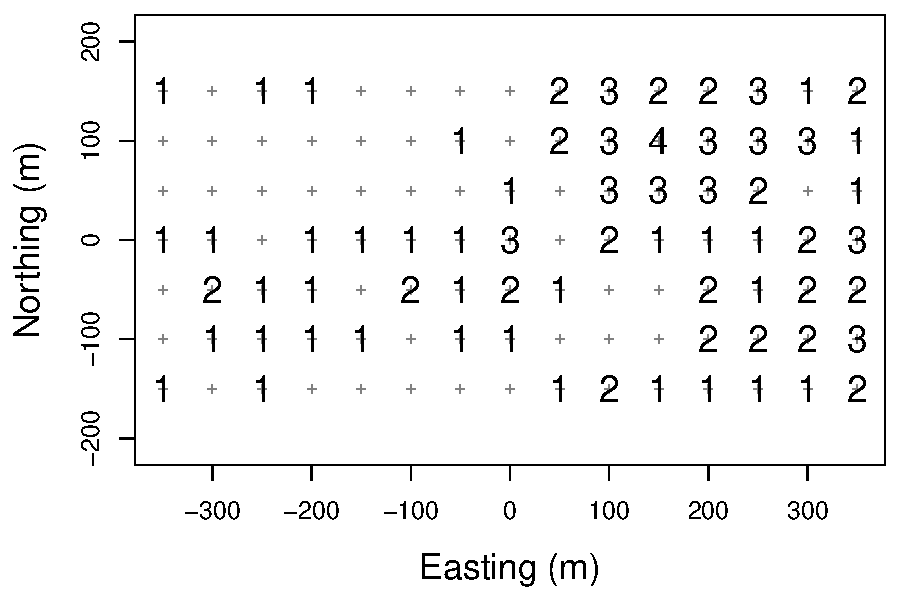
\includegraphics[width=0.9\textwidth]{Ch18-Unmarked/figs/nopaCounts}
  \caption{Spatially-correlated counts of northern parula. Gray
    crosses are the locations of the 105 point count
    stations. Superimposed are the number of detections after 3 survey occasions.}
  \label{fig:nopaDat}
\end{figure}


We used both versions of the code to fit the
model to the parula data. In our analyses, we defined the point process
state-space by buffering the grid of point count locations by 250 m,
and we set $M=200$. For inference, we generated three Markov chains,
each consisting of 300000 iterations after discarding the initial 10000
draws. %Convergence was satisfactory, as indicated by an $\hat{R}$
%statistic of $<$ 1.02 \citep{gelman_rubin:1992}.
\begin{small}
\begin{verbatim}
library(scrbook)
library(rjags)
data(nopa)
dat1 <- list(n = nopa$n, X = nopa$X, M=200, J=nrow(nopa$n), K=ncol(nopa$n),
             xlim=c(-600, 600), ylim=c(-400, 400))
init1 <- function() {
    n <- dat1$n
    J <- nrow(n); K <- ncol(n); M <- dat1$M
    y <- array(0L, c(M, J, K))
    for(j in 1:J) {
        for(k in 1:K) {
            y[sample(1:M, n[j,k]),j,k] <- 1
        }
    }
    list(y = y, sigma=rnorm(1, 100), lam0=0.5, z=rep(1, M))
}
pars1 <- c("sigma", "lam0", "N", "ED")
jm1 <- jags.model("nopa1.jag", dat1, init1, n.chains=3, n.adapt=500)
jc1 <- coda.samples(jm1, pars1, n.iter=31000)
\end{verbatim}
\end{small}




Because these models can take so long to run, we show \R~commands for
fitting the model using a single processor, and code for parallel
processing, which allows us to run 1 chain on each core. Obviously
your computer must have $>1$ core to do this, and you must have a
relatively recent version of \R~so that you can use the {\tt parallel}
package. First, the simple single-core code:




XXXX THE RESULTS OF THE TWO ANALYSES LOOK VERY SIMILAR AS EXPECTED XXXX

The posterior distribution for
$N$ was highly skewed with a long right tail resulting in a wide 95\%
credible interval (Table \ref{t:nopaPosts}). Nonetheless, the interval
for density, $D$, includes estimates reported from more intensive field
studies \citep{moldenhaer_regelski:1996}. As with any SCR model,
we can produce a density surface map, as shown in Fig.~\ref{fig:nopaDen}




\begin{table}%[t]
  \caption{Posterior summary statistics for spatial Poisson-count
    model applied to the northern parula data. Two sets of priors were
    considered. $M=200$ was used in both cases. Parulas/ha, $D$, is a
    derived parameter.}
  \scriptsize
  \begin{tabular}{l l rrrrrr}
    \hline
    Par        & Prior                  & Mean  & SD    & Mode   & q0.025  & q0.50  & q0.975  \\
    \hline
    $\sigma$   & $U(0, \infty)$   & 2.154   & 1.222  & 1.230   & 0.896   & 1.665   & 5.170    \\
    $\lambda_0$ & $U(0, \infty)$  & 0.284   & 0.149 & 0.212    & 0.084  & 0.256  & 0.665   \\
    $N$        & $U(0, M)$             & 40.953   & 38.072  & 4.000  & 3.000       & 31.000     & 143.000     \\
    $D$        &  --                   & 0.427    & 0.397 & 0.0417   & 0.0313  & 0.323  & 1.490    \\
    \hline
    $\sigma$    & $G(13, 10)$          & 1.301    & 0.258 & 1.230    & 0.889   & 1.266   & 1.908    \\
    $\lambda_0$ & $U(0, \infty)$ & 0.298    & 0.132 & 0.240    & 0.098   & 0.279  & 0.603   \\
    $N$         & $U(0, M)$            & 59.321   & 36.489  & 36.000 & 18.000      & 50.000     & 157.000     \\
    $D$         &  --                  & 0.618    & 0.380 & 0.375   & 0.188   & 0.521  & 1.635    \\
    \hline
  \end{tabular}
  \label{t:nopaPosts}
\end{table}


\begin{comment}

\begin{figure}
  \centering
  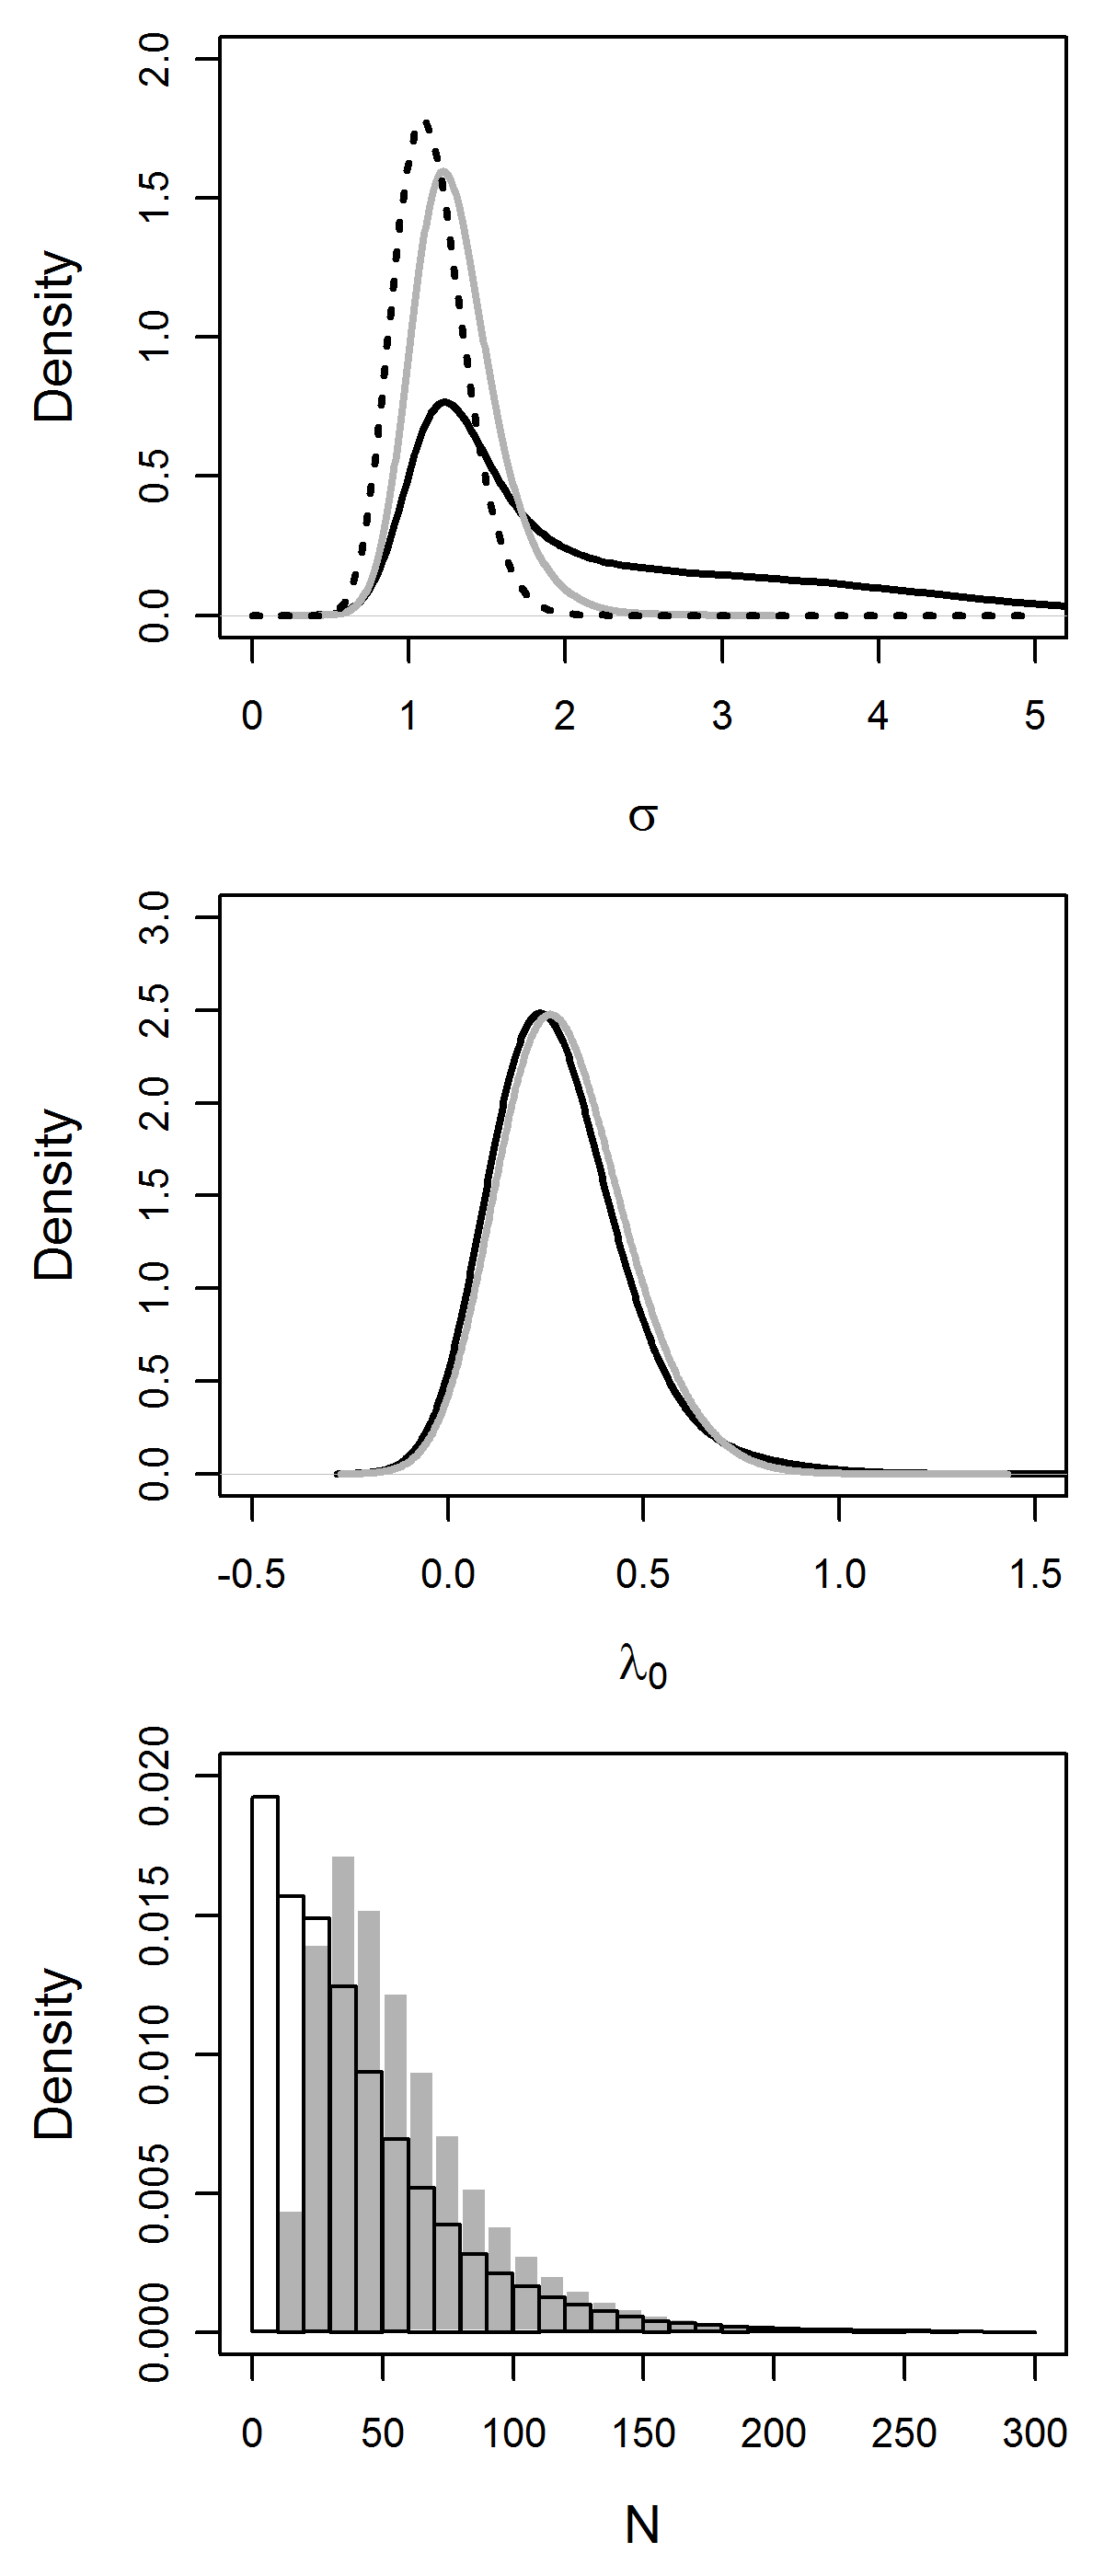
\includegraphics[width=1.5in,height=3in]{Ch18-Unmarked/figs/prior} % was 3,7
  \caption{Effects of $\sigma \sim \mbox{Gamma}(13,10)$
    prior on the posterior distributions from the northern parula
    model. Posteriors from model with uniform priors are
    shown in black, and posteriors from the informative prior model
    are shown in gray. The prior itself is shown as dotted line in the
    upper panel.}
  \label{fig:prior}
\end{figure}

\end{comment}


\begin{figure}
  \centering
  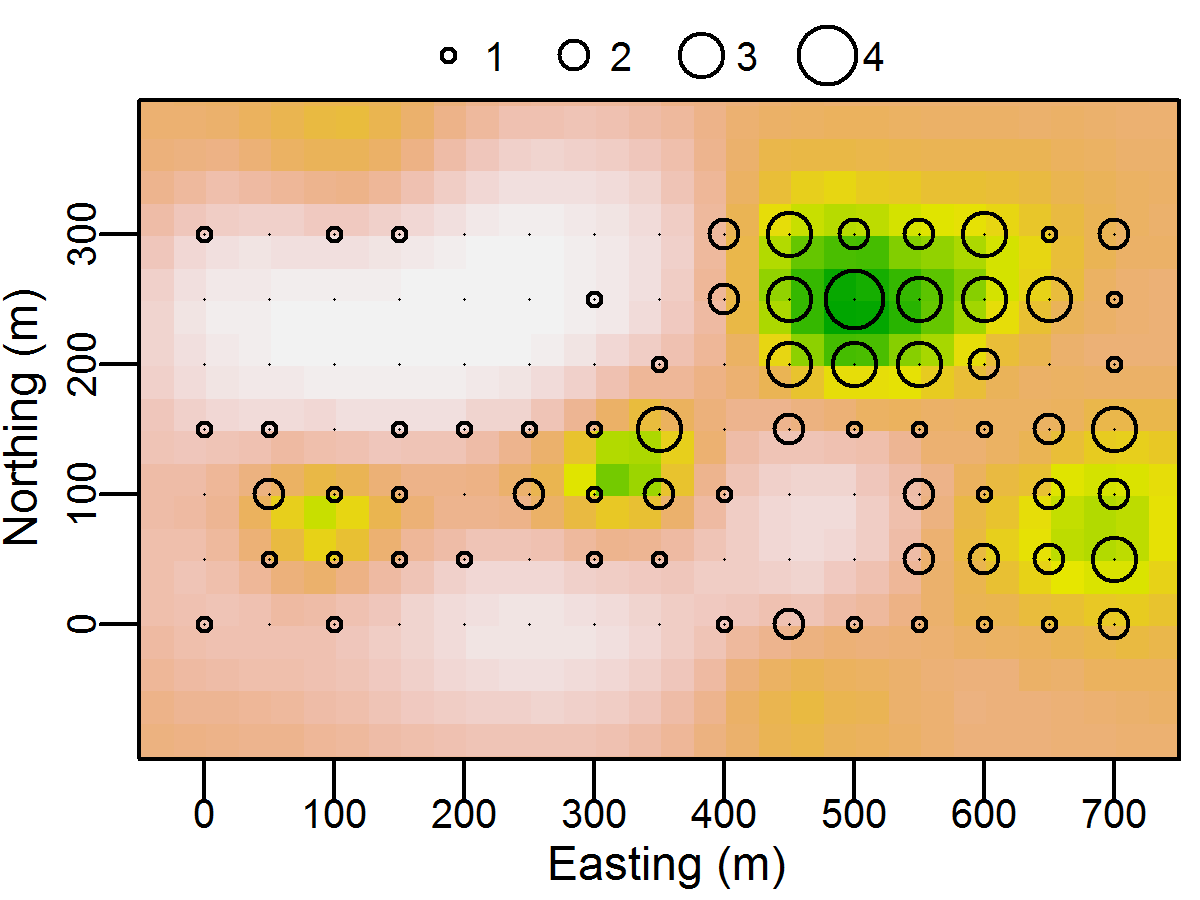
\includegraphics[width=3in,height=2.25in]{Ch18-Unmarked/figs/nopaDen}
  \caption{Estimated density surface of northern parula activity
    centers. The grid of point count locations with count totals is
    superimposed. See Fig. 1 for additional details.  }
  \label{fig:nopaDen}
\end{figure}

%\end{comment}



\section{Improving Precision with Prior Information}
\label{Sect.precision}

We are asking a lot of a little data. Because both the activity
centers and the encounter histories are latent variables, there is
inherently high uncertainty in the data, even if it is ``perfect''
data simulated from the true model. This explains the low posterior
precision in the parula data.

So why not just collect distance data or something? If you can, great---
we are not arguing against the use of other methods. But in many
cases, other models are not applicable. For instance, our model could
be applied to camera trapping data collected on species without
natural marks, such as pumas or coyotes. In addition, this
model provides an important foundation for modeling data where other
methods do not apply, and the underlying state model is so damn cool
because it corresponds to what we think is happening in the field.
Furthermore, the potential generalizations are numerous as we
will see later in this chapter and in the next chapter. In sum, the
model can be applied where no other models can, and it provides the
foundation for important extensions, but how can we improve precision?

Indeed, extensive information on home range size has
been compiled for many species in diverse habitats %\emph{e.g.}
\citep[\emph{e.g.},][]{degraaf_yamasaki:2001}. It is
easy to embody this information in a prior distribution as we
demonstrated for the parula data.


One benefit of a Bayesian analysis is that it can accommodate prior
information on the home range size and encounter rate parameters,
which are readily available for many
species. To illustrate, we analyzed the parula data using a new set of
priors. Whereas in the first analysis, all priors were
improper, customary non-informative priors (see Table \ref{t:nopaPosts}),
in the second set we used
an informative prior for the scale parameter $\sigma \sim
\mbox{Gamma}(13,10)$. We arrived at this prior using the methods
described by \citet{royle_etal:2011mee} and published
information on the warbler's home range size and detection probability
\citep{moldenhaer_regelski:1996,simons_etal:2009}. More details on this
derivation are found in ??????. We briefly note here that this prior
includes the biologically-plausible range of values from $\sigma$
suggested by the published literature.


This was true when considering
both sets of priors, although posterior precision was higher under the
informative set of priors. Specifically, the use of prior information
reduced posterior density at high, biologically implausible,
values of $\sigma$, and hence decreased the posterior mass for
low values of $N$ (Fig.~\ref{fig:prior}).


\subsection{Similarity to other data augmentation schemes}

By including the $w$ variables in the model, we have made use of the
data augmentation technique introduced by \citet{royle_etal:2007} and
developed by \citep{royle:2009} and
\citep{royle_dorazio:2010}. However, including the latent encounter
histories in the model can also be viewed as another form of data
augmentation, which was in fact, first proposed as a general model of
spatial dependence in count data
\citep{wolpert_ickstadt:1998}.

The model of
\citet{wolpert_ickstadt:1998} is slighly different than the SC model
in that they defined $\{{\bf s}_1, \ldots, {\bf s}_N\}$ not as a
realization from a spatial point process, but rather as locations of a
dense array of points, typically a fine grid covering the $J$ survey
locations. The purpose of this grid is to introduce random spatial noise into the system,
which is then smoothed using what, in our case, is the encounter
model. In their case, the encounter model is simply a smoothing
kernel that determines the spatial covariance structure -- if $\sigma$
is high relative to the ``trap'' spacing, the counts will be highly
correlated, and vice versa. Similar ideas have been used to model
spatial dependence in temperature data \citep{higdon:1998}. In the SC
model, $\sigma$ and the encounter model also determine the spatial
correlation, but it has an explicit connection to
correlation as information about the number and location of the
activity centers.

In addition to the fact that they fixed
the locations of the $\bf s$'s, their model also differs from the SC
model in that they also fix $N$, it being chosen to create a suitably
fine grid for generating the white noise.



\section{Design issues}

\subsection{How Much Correlation Is Enough?}

$\sigma$ shouldn't be too small or too large relative to trap spacing.

Can we test for correlation using K-functions or something?

\subsection{Linear Designs}

Survey points are not always located on a grid with even spacing---in
fact, it is rare to see a perfect 10$\times$10 grid of points in any
study because of habitat patchiness or rugged terrain or what have
you. Instead, points are often distributed haphazardly or using some form of
probability sampling. Such designs can still produce data amenable to
the models we consider in this chapter if individuals can be
encountered at multiple points, and none of the considerations
discussed above need to be modified. But what about linear designs?

In bird studies, point counts are often placed on linear transects. For
example, the Breeding Bird Survey involves surveying 50 points spaced
by 0.5 miles. The mountain-top bird survey in the White Mountain
National Forest involves surveying 42 transects, each with 20? points
spaced by 250-m \citep{king_etal:2008}. For many species, the 0.5 mile
spacing of the BBS will ensure that individuals are not detected at
multiple points. However, in the moutain-top survey, it's easy to
imagine that a Bicknell's Thrush (\emph{Catharus bicknelli}) could
easily be heard from adjacent points. So can we apply our model to
obtain density estimates with such simple counts?



\subsection{Quadrat counts}





\section{Alternative Observation Models}
\label{Sect.alt-obsmods}

\citet{chandler_royle:2012} focused exclusively on the Poisson
observation model, but noted that alternative models such as the
Bernoulli model or the multinomial model (Chapt. \ref{chapt.poisson-mn}) should
be easily accomodated. Unfortunately, our experimentation with these models
indicates that the base-line encounter probability parameter $p_0$ is
not identifiable. At this point in time, it is not clear why this
would be so. However, this situation is similar to that of traditional
mark-resight models where the unmarked individuals provide no
information about the parameters of the capture process. Under these
models, capture or re-sight probability can only be estimated by
marking a subset of the population. In the next chapter we demonstrate
how data from marked and unmarked individuals can be combined to
improve precision and allow for the estimation of parameters under the
alternative observation models.



\subsection{Spatial point process models}


Our model has some direct linkages to existing point process
models. We note that the observation intensity function (i.e.,
corresponding to the observation
locations) is a compound Gaussian kernel similar to
that of the Thomas process
\citep[pp. 61-62]{thomas:1949, moller_waagepetersen:2004}.
Also, the Poisson-Gamma Convolution models
\citep{wolpert_ickstadt:1998} are structurally similar (see also \cite{higdon:1998}
and \cite{best_etal:2000}).
 In particular, our model is such a model but
with a {\it constant} basal encounter rate $\lambda_{0}$
and {\it unknown} number and location of ``support points'', which in
our case are the animal activity centers, $\bf{s_i}$.
We can thus regard our model as a model for
{\it estimating} the location and local density of support points in
such models, which we believe could be useful in the application of
convolution models.  \citet{best_etal:2000} devise an MCMC algorithm for the
Poisson-Gamma model based on data augmentation, which is
similar to the component of our algorithm for
updating the $z$ variables in
the conditional-on-$z$ formulation of the model.  We emphasize that
our model is distinct from these Poisson-Gamma models
in that the number {\it and} location of such
support points are estimated.


If individuals were perfectly observable then the resulting point
process of locations is clearly a standard Poisson or Binomial (fixed
$N$) cluster process or Neyman-Scott process.
If detection is uniform over space but
imperfect, then the basic process is unaffected by this random thinning.
Our model can therefore be viewed formally as a Poisson (or Binomial)
cluster process model but one in which the thinning is
non-uniform, governed by the encounter model which dictates that
thinning rate increases with distance from the observation points. In
addition, our inference objective is, essentially, to estimate the
number of parents in the underlying Poisson cluster
process,
where the observations are biased by an incomplete sampling apparatus
(points in space).


As a model of a thinned point process, our model has much in common
with classical distance sampling models \citep{buckland_etal:2001}.
The main distinction is that our data structure does {\it not} include
observed distances, although the underlying observation model is
fundamentally the same as in distance sampling if there is only a
single replicate sample and $\bf{s}_i$ is defined as an individual's
location at an instant in time. For replicate samples, our model preserves
(latent) individuality across samples and traps which is not a feature
of distance sampling. We note that error in measurement of distance is
not a relevant consideration in our model, and we explicitly do not
require the standard distance sampling assumption that the probability
of detection is 1 if an individual occurs at the survey point. More
importantly, distance sampling models cannot be applied to data from
many of the sampling designs for which our model is relevant. For
example, many rare and endangered species can only be
effectively surveyed using methods such as hair snares and camera
traps that do not produce distance data \citep{oconnell_etal:2010}.


\section{Summary and Outlook}

The SC model is a conceptually simple extension of standard SCR
models, but in terms of computational requirements and latent
structure, it is perhaps at the extreme end of what is possible to do
with count data. As is always true, we must recognize that
our models can never exactly depict the complexities of natural
systems, and so we must decide how what level of complexity is
sufficient for our purposes...

At the other end of the spectrum is perhaps a simple Poisson
regression. We sum up the counts at each trap and fit a model using a
function like \verb+glm+. But what would be estimating?

Concerns about ``statistical independence'' have prompted
ecologists to design count-based studies such that observed
random variables can be regarded as {\it i.i.d.} outcomes
\citep{hurlbert:1984}. Interestingly, this
often proves impossible in practice, and elaborate
methods have been devised to model spatial dependence as a nuisance
parameter. Our paper presents a modeling framework that directly
confronts this view by demonstrating that spatial
correlation carries information about the locations of individuals,
which can be used to estimate density even when individuals
are unmarked and distance-related heterogeneity exists in encounter
probability.




It is also interesting to note that by disregarding individual
identity, we wind up with a model that closely resembles another large
class of spatial models, known as convolution models
\citep{wolpert_ickstadt:1998,higdon:1998}. These
models have been used for a variety of purposes such as describing oceanic
surface temperatures and correlation in tree locations within managed
forests. The SC model offers an improvement in
some respects over existing convolution models because it does not
require arbitrary decisions about the location and number of ``support
points''. We will clarify this later in the chapter, and briefly
mention how this model can be used outside of SCR contexts for general
purpose spatial modeling of correlated count data.


In this paper, we confronted one of the most difficult challenges
faced in wildlife sampling ---
estimation of density in the absence of data to distinguish among
individuals. To do so, we developed a novel class of
spatially-explicit models that
applies to spatially organized counts, where the count locations or
devices are located sufficiently close together so that individuals
are exposed to encounter at multiple devices. This design yields
correlation in the observed counts, and this correlation proves to be
informative about encounter probability parameters and hence density.
We note that sample locations in count-based studies are typically
{\it not} organized close
together in space because conventional wisdom and standard practice
dictate that independence of sample units is necessary
\citep{hurlbert:1984}. Our model
suggests that in some cases it might be advantageous to deviate from
the conventional wisdom if one is interested in direct inference about
density. Of course, this is also known in the application of standard spatial
capture-recapture  models \citep{borchers_efford:2008}
where individual
identity is preserved across trap encounters, but it is seldom, if
ever, considered in the design of more traditional count surveys.

Our model has broad relevance to an incredible number of animal
sampling problems. Our motivating problem involved bird point counts
where individual
identity is typically not available. The model also applies
to other standard methods used to sample unmarked
populations,  such as camera traps
or even methods that yield sign ({\it e.g.} scat, track) counts
indexed by space. However, results of our simulation study reveal some
important limitations of the basic
estimator applied to situations in which none of the individuals can
be uniquely identified. In particular, posterior
distributions are highly skewed in typical small to moderate sample
size situations and posterior precision is low.

